\chapter{Introduction}
\label{Introduction}

\section{Purpose}
This document is a specification of the Remote Interoperability Protocol (RIP), which was conceived at UNED for the remote operation of online laboratories (OLs). Instructions on how to correctly implement both a server and a client that talk RIP are also given.

\section{Document Conventions}
For the purpose of this document, we consider that an OL can either be a virtual laboratory (VL) or a remote laboratory (RL).

VLs are simulations and offer experimentation possibilities based on mathematical models.

RLs use lab equipment and perform the experiments in real life, just remotely.

A \textit{simulation model} is understood as software that includes mathematical models that simulates a system for virtual experimentation purposes.

\textit{Control program} is a term used in this document to refer to the software in charge of controlling and monitoring lab equipment.

In this sense, we consider that a VL always has an associated \textit{simulation model} that is hosted and run in some computer, while a RL always has an associated \textit{control program} that is also hosted and run in some computer.

Finally, we define an \textit{experience} as each of the lab activities that can be carried out with an OL implementation, either through a RL or through a VL.

\section{Intended Audience and Reading Suggestions}
Audiences that may be interested in this document are educators, researchers and industry stakeholders that want or need to remotely communicate either with hardware devices or mathematical models from a web application. 

More specifically, this document aims at anyone who is interested in one or more of the following points:

\begin{enumerate}
    \item Implementing a RIP server and/or a RIP client to use RIP as the communication protocol for operating OLs.
    \item Using or modifying an existing RIP server and/or RIP client implementation.
    \item Making modifications on the RIP protocol itself.
\end{enumerate}

In any of the above cases, it is advised to read the present document in order. Before reading this document, it is reccommended to have some notions about TCP \cite{tcp}, HTTP \cite{http}, SSE \cite{sse} and JSON-RPC \cite{jsonrpc}.

\section{Product Scope}
The objective of RIP is to offer a simple, yet powerful, communication solution usable from web clients. As such, RIP only uses pure HTTP standard protocols, supported by all major web browsers.

RIP is designed to communicate web clients with OLs; either VLs or RLs. When used to communicate with a VL, RIP exposes meta-data and input and output methods and variables related to a simulation model that is hosted and runs on a computer (usually, a remote server). When used to communicate with a RL, RIP does the same thing with a \textit{control program} defined in a computer (usually, a remote server) to monitor and manipulate the lab equipment.

Figure \ref{fig:Client-RIP-OL} shows the usage of the RIP protocol implemented in a RIP client and a RIP server to communicate a web client with an OL. The figure represents how an OL can implement either a VL, a RL, or any combination of both, each one defined as an independent \textit{experience}, referenced through a certain \textit{expid} parameter.

\begin{figure}
\centering
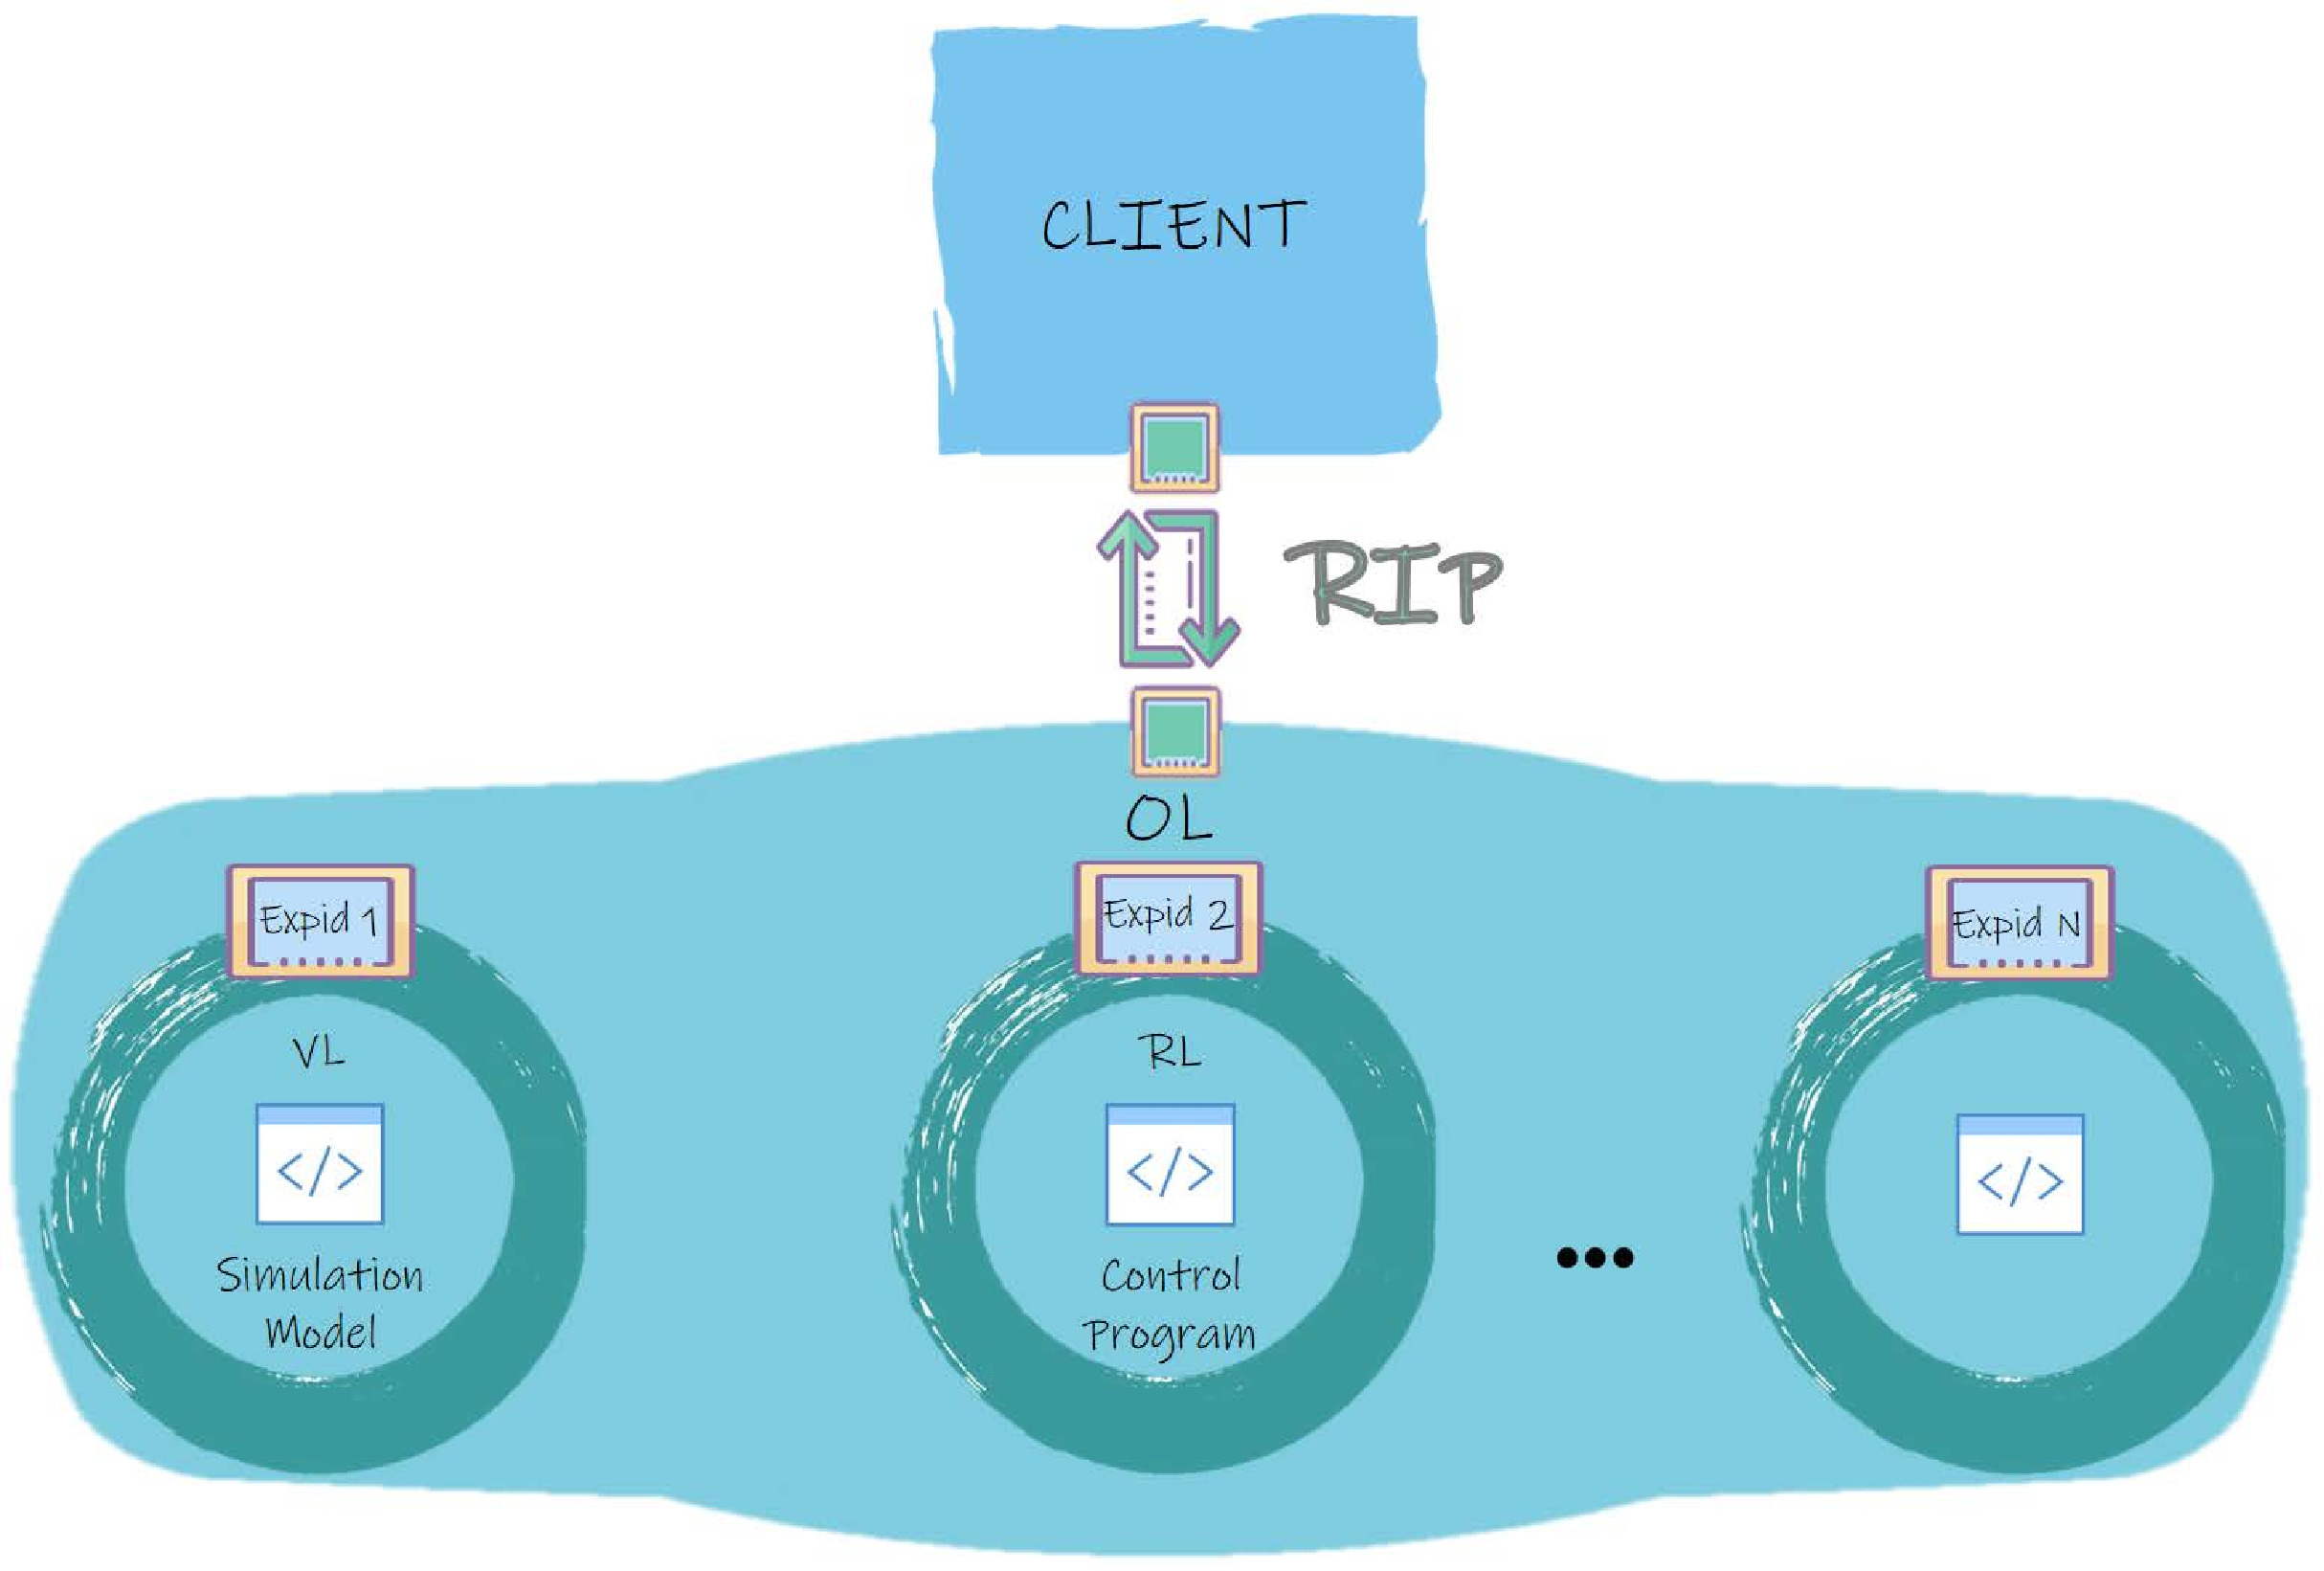
\includegraphics[width=0.75\textwidth]{images/Client-RIP-OL.pdf}
\caption{RIP protocol is used by a RIP client and a RIP server to communicate both. The RIP server is implemented in an OL and the RIP client is implemented in a web browser application.}
\label{fig:Client-RIP-OL}
\end{figure}


\chapter{Overall Description}
\label{Overall Description}

\section{Protocol Perspective}
The protocol is an open source, under the GNU general Public License. It is a communication protocol to be used in the client-server model, especially designed for OLs in which the client runs within a web browser. RIP provides a simple mechanism for users and client machines/programs to acquire information about the lab \textit{experiences} defined in the server and about each \textit{experience's} inputs and outputs. The protocol also defines methods for reading and writing the values of these inputs and outputs, respectively.

\begin{figure}[b!]
\centering
\includegraphics[width=0.5\textwidth]{images/RIPTechnologies.pdf}
\caption{RIP is based on POST and GET HTTP methods and on the JSON-RPC format.}
\label{fig:RIP_Technologies}
\end{figure}

The main features of RIP are the following:

\begin{enumerate}
    \item Defining \textit{experiences} on the OL.
    \item Obtaining meta-data related to each defined \textit{experience}.
    \item Obtaining a list of readable and writable variables for each \textit{experience}.
    \item Obtaining a list of methods to read and write variables in each \textit{experience}.
    \item Invoking methods to read and write variables in each \textit{experience}.
    \item Defining server events to send data either periodically or based on any other triggering condition defined in an \textit{experience}.
    \item Subscribing a client to any server event declared in an \textit{experience}.
\end{enumerate}

RIP is based on two cornerstones: POST and GET methods for the communications transport and JSON-RPC for formatting messages. POST and GET are HTTP methods, which, in turn, is based on TCP communications. On the other hand, JSON-RPC is based on the JSON format. Figure \ref{fig:RIP_Technologies} represents these ideas.

Communication between two software entities is possible when they talk the same protocol. Therefore, a RIP implementation is needed in both the client and the server.

\subsection{Server Implementation Perspective}
Figure \ref{fig:RIP_Architecture} depicts the architecture of a \emph{RIP Server} that implements the RIP protocol. To sum it up, there are three functional subsystems: the \emph{Web Server}, that handles client connections, user sessions, etc., the \emph{command interpreter}, that speaks RIP, and the \emph{executor}, that controls the execution of the laboratory \textit{control programs} or \textit{simulation models}.

\begin{figure}
\centering
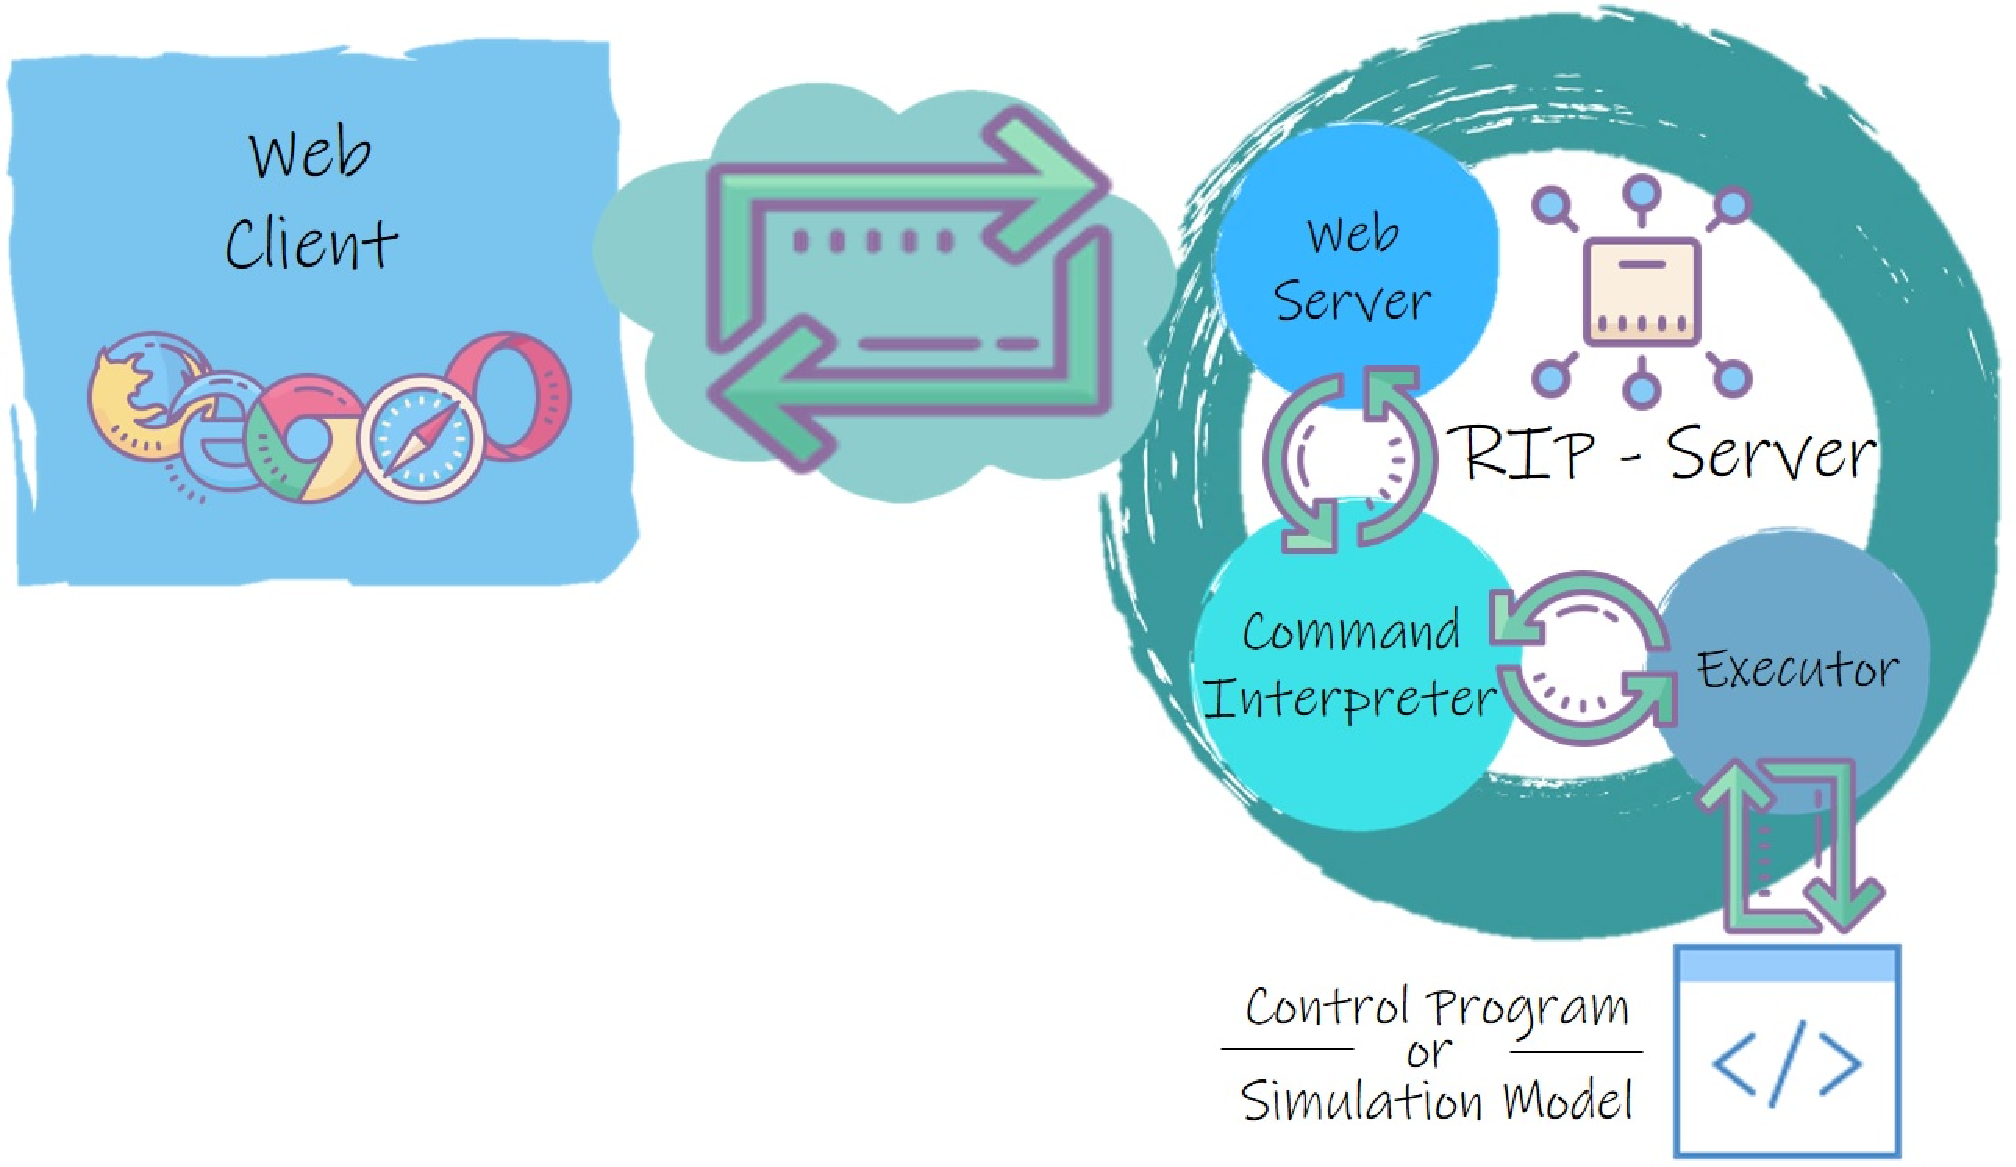
\includegraphics[width=0.75\textwidth]{images/RIPArchitecture.pdf}
\caption{Architectural view of a RIP Server}
\label{fig:RIP_Architecture}
\end{figure}

The Web Server admits (and handles in different ways) three types of requests: GET (used to retrieve \textit{experiences'} meta-data), SSE (used to get server-to-client data updates) and POST (used to send client-to-server updates or client-to-server requests for data updates). These different methods are each associated with the three basic cases of use, namely:

\begin{itemize}
    \item \emph{Meta-data} - A client, wanting to obtain information about the laboratory, launches an HTTP GET request to the URL associated with the laboratory. The RIP server responds with a JSON-RPC structure that informs the client, depending on the request's parameters, with one of the following:
    
    \begin{enumerate}
        \item General information about the OL: what are the \textit{experiences} defined and how they can be accessed.
        \item Detailed information of a particular \textit{experience} (when the request includes the {experience} id as a parameter).
    \end{enumerate}
    
    \item \emph{Observer} - A client, that desires to receive updates on the state of the plant, subscribes to an SSE event stream associated to the \textit{experience} of interest.
    
    \item \emph{Operator} - A client, wanting to act over the OL or to receive an update on demand, sends a POST request with the command codified as a RIP-JSON-RPC structure.
\end{itemize}

An \textit{experience} represents a lab activity associated with an OL. In the case of RLs, each \textit{experience} is implemented as a \textit{control program}, which in general is responsible of managing the physical connections with the hardware, safe measures, and any other functionality the lab designer has considered appropriate to include. In the case of VLs, each \textit{experience} is implemented as a \textit{simulation model} that represents a real system. The \textit{experience} abstraction is useful for two purposes: 1) to publish information about OLs in a standard and structured way and 2) to allow for hosting and running several different \textit{control programs} or \textit{simulation models} in the same computer.

\subsection{Client Implementation Perspective}
A RIP client must simply implement the required communication protocol methods (that is, POST, GET and SSE) with the appropriate format for reading and writing the messages content (that is, JSON-RPC) and the structure and functions defined by RIP (detailed in later sections).

\section{Protocol Functions (High-Level API)}
The functions defined and used in the protocol are divided in two types: internal and external.

The internal functions are private functions, not exposed to the web clients. These methods are used internally by RIP server implementations to communicate either with the \textit{simulation model} or the \textit{control program} used in the OL.

The external functions are exposed through web services as public functions, and so, they are callable by the web clients. These methods are used by the RIP servers and clients to both get meta-data about the defined \textit{experiences} and to write and read data to and from the OL.

In this way, RIP servers must implement both the internal and the external functions while RIP clients must implement only the external functions (see Figure \ref{fig:Functions_Implementation}).

\begin{figure}
\centering
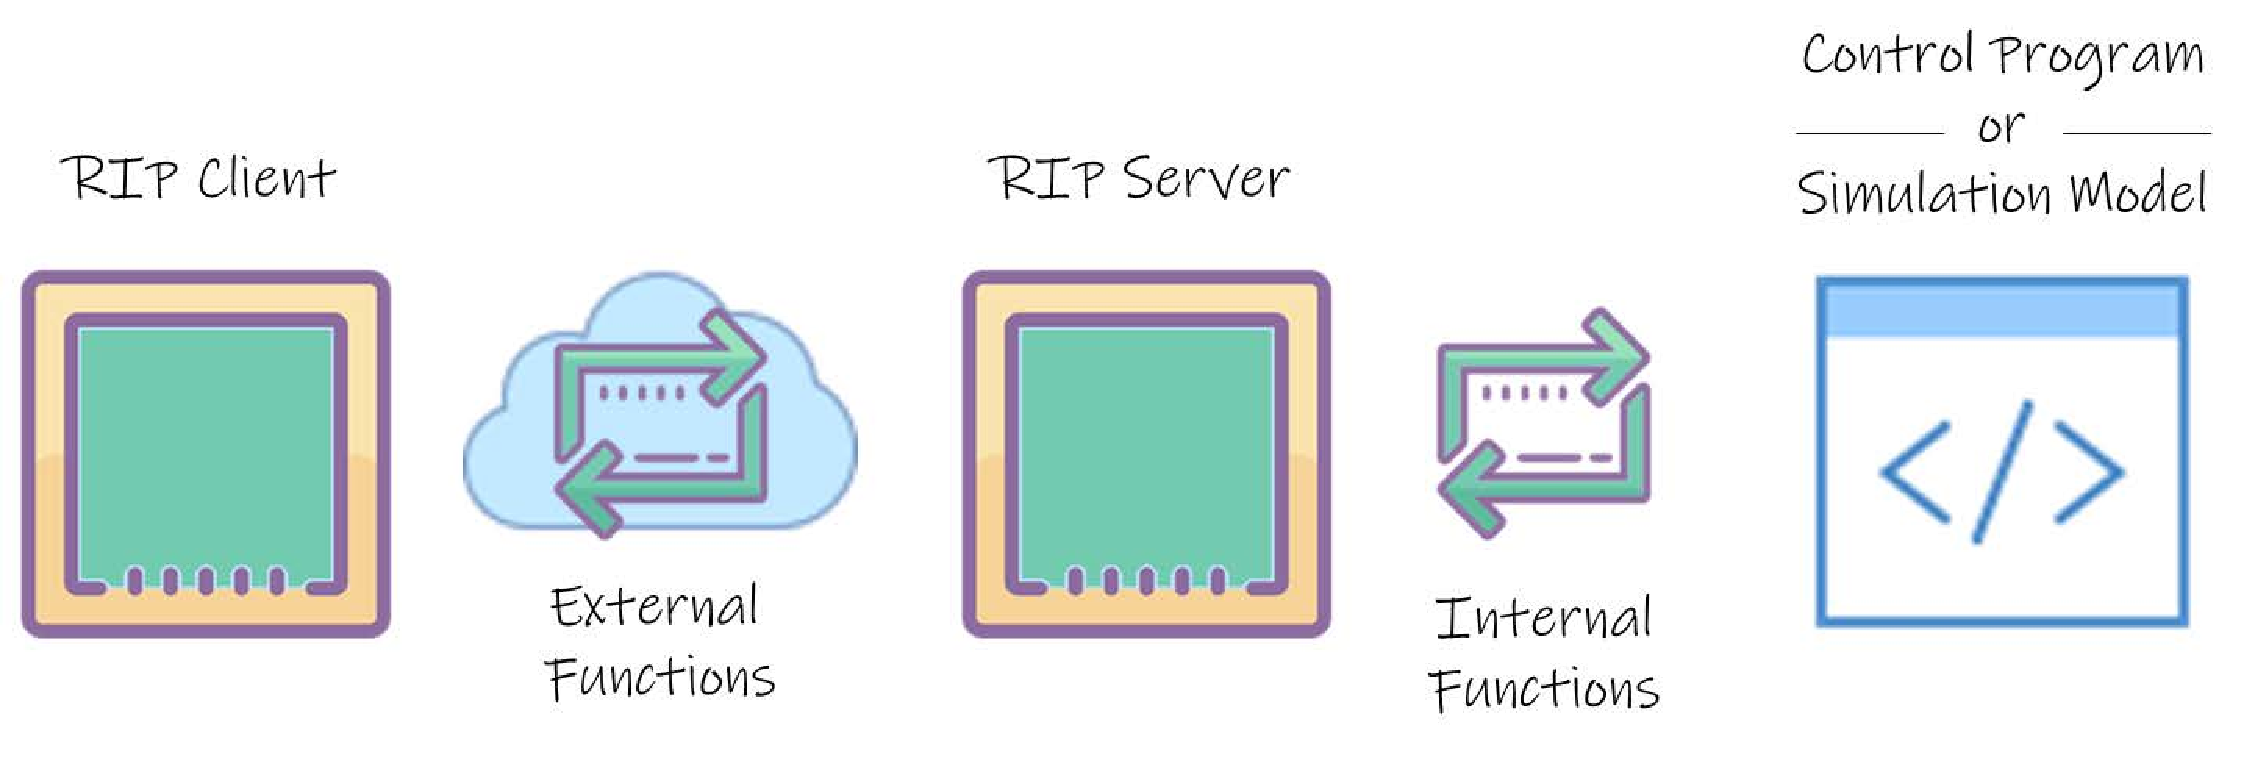
\includegraphics[width=0.75\textwidth]{images/FunctionsImplementation.pdf}
\caption{Internal and external functions implementation in RIP clients and servers}
\label{fig:Functions_Implementation}
\end{figure}

\subsection{Internal Functions}
\label{sec:Internal_Functions}
The list of existing internal functions a RIP server must implement is:

\begin{enumerate}
    \item \textit{readablelist}, \textit{writablelist}  $=$ \textbf{open}(\textit{expid}): Returns the list of readable and writable variables (in two different variables) defined in the \textit{experience} associated to the input \textit{expid} parameter.
    \item \textbf{close}(\textit{expid}): Closes the control program (if it is a RL) or the simulation model (if it is a VL) of the OL \textit{experience} defined by the input \textit{expid} parameter.
\end{enumerate}

\subsection{External Functions}
\label{sec:External_Functions}
The list of existing external functions a RIP server must implement so that a RIP client may use is:

\begin{enumerate}
    \item \textbf{info}(\textit{expid} = null): Retrieves the meta-data information about the \textit{experience} defined by the input \textit{expid} parameter.  This parameter is optional and if it is not specified, the method then returns meta-data information about all the \textit{experiences} defined.
    \item \textbf{start}(\textit{expid}): Starts the execution of the control program (if it is a RL) or the simulation model (if it is a VL) of the OL \textit{experience} associated to the input \textit{expid} parameter.
    \item \textbf{stop}(\textit{expid}): Stops the execution of the control program (if it is a RL) or the simulation model (if it is a VL) of the OL \textit{experience} defined by the input \textit{expid} parameter.
    \item \textit{readvariablenames}, \textit{readvariablevalues} $=$ \textbf{get}(\textit{expid}, \textit{variablenames}): Retrieves the current values of the variables (\textit{readvariablevalues}) specified by the \textit{variablenames} input parameter. For this to happen, these variables must exist in the \textit{control program} or \textit{simulation model} associated to the \textit{experience} defined by the \textit{expid} input parameter. When the \textbf{get()} method is called, \textit{readvariablenames} contains only the names of the variables that were successfully read, not all requested ones in \textit{variablenamess}.
    \item \textbf{set}(\textit{expid}, \textit{variablenames}, \textit{variablevalues}): Writes the received values (\textit{variablevalues}) in the specified variables (\textit{variablenames}) of the appropiate OL \textit{experience}. For this to happen, these variables must exist in the \textit{control program} or \textit{simulation model} associated to the (\textit{expid}) input parameter.
\end{enumerate}

Where:

Variables \textit{variablenames} and \textit{variablevalues} are arrays of text. For example: \textit{variablenamess} $=$ ["x", "y", ...], \textit{variablevalues} $=$ ["10", "a", ...].

Each method returns an error indicator when the operation is not completed successfully.

At the moment, only numbers, text and booleans are supported in the \textbf{set}() and \textbf{get}() methods.

\section{Protocol Communication Methods (Low-Level API)}
Three HTTP communication methods are available in RIP:

\begin{enumerate}
    \item \textbf{GET} - To obtain OL meta-data.
    \item \textbf{POST} - To send client-to-server requests for (i) writing OL variables' values and (ii) reading OL variables' values.
    \item \textbf{SSE} - To subscribe the client to data streams so that it receives server-to-client OL variables' values updates.
\end{enumerate}

Table \ref{tab:low-high-levels-correspondence} shows the correspondence between the external protocol functions of the high-level API and the HTTP methods of the low-level API:

\begin{table}[]
    \centering
    \begin{tabular}{|c|c|}\hline
         &  \\HTTP Method & RIP function \\\hline
         &  \\GET & info(), info(expid) \\\hline
         &  \\POST & set(), get(), start(), stop() \\\hline
         &  \\SSE & TODO \\\hline
    \end{tabular}
    \caption{RIP functions - HTTP methods correspondence}
    \label{tab:low-high-levels-correspondence}
\end{table}

\section{Operating Environment}
RIP uses only HTTP methods for the communication. Therefore, it works in any major web browser. However, RIP also relies on the use of SSEs, which, up to date, are not supported by Microsoft Internet Explorer nor Microsoft Edge. Nevertheless, there are numerous poly-fill solutions for implementing SSE so that they work on these browsers that do not support them natively.

\section{Design and Implementation Constraints}
RIP is designed to only use pure HTTP methods on purpose, with the aim of guaranteeing its correct functioning from web browsers. Therefore, the only hard implementation constraint is that HTTP is used for implementing RIP communications.

\section{Assumptions and Dependencies}
RIP depends solely on the use of HTTP POST and GET methods and on the JSON format for exchanging data. 

A common and easy way of implementing RIP in web clients is through the use of the EventSource object \cite{eventsource} (for the SSEs) and the XMLHTTPRequest object \cite{xhr} or the Fetch API \cite{fetch} (for the POST messages), which are both supported by all major web browsers. Still, implementations without the use of such APIs are possible, just more laborious. 

RIP server implementations may differ a lot depending on the language used to make the implementation, and so do their possible dependencies.

\section{User Documentation}
This section provides a deeper insight on the high-level API, which is the only knowledge required by a user to use a RIP client implementation to communicate with an OL running a RIP server.

A RIP client must implement a class with the methods described in Section \ref{sec:External_Functions}. Next, detailed information of the result returned by each method is given.

\subsection{Method info}
This method can be called with or without the \textit{expid} input parameter.

When called without this parameter, \textbf{info()} returns meta-data with the list of experience identifiers associated to all \textit{experiences} defined in the OL. It also returns more information about the low-level API method call for retrieving meta-data. The result is a JSON object containing one single top-level member:

\begin{enumerate}
    \item \textbf{experiences}: A JSON object with the following top-level members:
    \begin{enumerate}
        \item \textbf{list}: An array of JSON objects, each of which contains one single top-level member:
        \begin{enumerate}
            \item \textbf{id}: A string with the experience identifier (expid) that is unmistakably related to one and only one \textit{experience} defined in the OL.
        \end{enumerate}
        \item \textbf{methods}: An array of JSON objects, each of which contains the following top-level members:
        \begin{enumerate}
            \item \textbf{url}: A string with the URL to call the method.
            \item \textbf{type}: A string specifying the HTTP method to use.
            \item \textbf{description}: A string describing the method.
            \item \textbf{params}: An array of JSON objects detailing the required and optional parameters for the method:
            \begin{enumerate}
                \item \textbf{name}: A string with the name of the parameter
                \item \textbf{required}: A string ("yes" or "no") specifiying whether the parameter is required ("yes") or optional ("no").
                \item \textbf{location}: A string referencing the location for the parameter ("header", "query" or "body").
                \item \textbf{value}: [Optional] A string with the required value for the parameter.
                \item \textbf{type}: [Optional] A string detailing the type of the parameter.
            \end{enumerate}
            \item \textbf{returns}: A string with the MIME-type of the method's result.
            \item \textbf{example}: A string with an example on how to call the method.
        \end{enumerate}
    \end{enumerate}
\end{enumerate}

Example:

\begin{lstlisting}
{
  "experiences": {
    "list": [
              {
              "id": "Test1"
              },
              {
              "id": "Test2"
              }
            ],
    "methods": [
                  {
                  "url": "10.192.38.68:8080/RIP",
                  "type": "GET",
                  "description": "Retrieves information (variables and methods) of the experiences in the server",
                  "params": [
                               {
                               "name": "Accept",
                               "required": "no",
                               "location": "header",
                               "value": "application/json"
                               },
                               {
                               "name": "expId",
                               "required": "no",
                               "location": "query",
                               "type": "string" 
                               }
                            ],
                  "returns": "application/json",
                  "example": "10.192.38.68:8080/RIP?expId=Test1"
                  }
               ]
    }
}
\end{lstlisting}

When called with the \textit{expid} parameter, \textbf{info(expid)} returns meta-data of the referenced \textit{experience}. The result is a JSON object containing three top-level members:

\begin{enumerate}
    \item \textbf{info}: TODO
    \item \textbf{readables}: TODO
    \item \textbf{writables}: TODO
\end{enumerate}

Example:

\begin{lstlisting}
{
"info": {
        "name": "Test1",
        "description": "Test1",
        "authors": "L. de la Torre",
        "keywords": ["Test", "Example"]
        },
"readables": {
    "list": [
               {
               "name": "intout",
               "description": "integer outputs",
               "type": "int",
               "min": "-2147483648",
               "max": "2147483647",
               "precision":"1"
               },
               {
               "name": "stringout",
               "description": "String output",
               "type": "string",
               "min": "",
               "max": "",
               "precision": ""
               },
               {
               "name": "booleanout",
               "description": "Boolean output",
               "type": "boolean",
               "min": "false",
               "max": "true",
               "precision":""
               },
               {
               "name": "doubleout",
               "description": "double output",
               "type": "float",
               "min": "-Inf",
               "max": "Inf",
               "precision": "0"
               }
            ],
    "methods": [  
                  {
                  "url": "10.192.38.68:8080/RIP/SSE",
                  "type": "GET",
                  "description": "Suscribes to an SSE to get regular updates on the servers' variables",
                  "params": [
                               {
                               "name": "Accept",
                               "required": "no",
                               "location": "header",
                               "value": "application/json"
                               },
                               {
                               "name": "expId",
                               "required": "yes",
                               "location": "query",
                               "type": "string"
                               },
                               {
                               "name": "variables",
                               "required": "no",
                               "location": "query",
                               "type": "array",
                               "subtype": "string"
                               }
                            ],
                  "returns": "text/event-stream",
                  "example": "10.192.38.68:8080/RIP/SSE?expId=TestOK"
                  },
                  {
                  "url": "10.192.38.68:8080/RIP/POST",
                  "type": "POST",
                  "description": "Sends a request to retrieve the value of one or more servers' variables on demand",
                  "params": [
                               {
                               "name": "Accept",
                               "required": "no",
                               "location": "header",
                               "value": "application/json"
                               },
                               {
                               "name": "Content-Type",
                               "required": "yes",
                               "location": "header",
                               "value": "application/json"
                               },
                               {
                               "name": "jsonrpc",
                               "required": "yes",
                               "type": "string",
                               "location": "body",
                               "value": "2.0"
                               },
                               {
                               "name": "method",
                               "required": "yes",
                               "type": "string",
                               "location": "body",
                               "value": "get"
                               },
                               {
                               "name": "params",
                               "required": "yes",
                               "type": "array",
                               "elements": [
                                   {
                                   "description": "Experience id","type":"string"},{"description":"Name of variables to be retrieved",
                                   "type": "array",
                                   "subtype": "string"
                                   }
                                ],
                              "location": "body"
                              },
                              {
                              "name": "id",
                              "required": "yes",
                              "type": "int",
                              "location":"body"
                              }
                            ],
                  "returns": "application/json",
                  "example": {
                             "10.192.38.68:8080/RIP/POST": 
                             {
                             "headers": {
                                        "Accept": "application/json",
                                        "Content-Type": "application/json"
                                        },
                             "body": {
                                     "jsonrpc": "2.0",
                                     "method": "get",
                                     "params": [
                                                  "TestOK",
                                                  ["var1","var2"]
                                               ],
                                     "id":"1"
                                     }
                             }
                            }
                  },
                  {
                  "url": "http://camera1_ip/axis-cgi/mjpg/video.cgi",
                  "type": "GET",
                  "description": "Retrieve an image of the lab captured from the camera: 'Camera 1'",
                  "params": [
                               {
                               "name": "resolution",
                               "required": "no",
                               "location": "query",
                               "type": "string"
                               },
                               {
                               "name": "user",
                               "required": "no",
                               "location": "query",
                               "type": "string"
                               },
                               {
                               "name": "password",
                               "required": "no",
                               "location": "query",
                               "type": "string"
                               }
                            ],
                  "returns": "video/x-motion-jpeg",
                  "example": "http://camera1_ip/axis-cgi/mjpg/video.cgi"
                  }
               ]
             },
"writables": {
    "list": [
               {
               "name": "intin",
               "description": "integer imput",
               "type": "int",
               "min": "-2147483648",
               "max": "2147483647",
               "precision":"1"
               },
               {
               "name": "stop",
               "description": "Stops the Vi",
               "type": "boolean",
               "min": "false",
               "max": "true",
               "precision":""
               },
               {
               "name": "booleanin",
               "description": "Boolean input",
               "type": "boolean",
               "min": "false",
               "max": "true",
               "precision": ""
               },
               {"name": "stringin",
               "description": "String input",
               "type": "string",
               "min": "",
               "max": "",
               "precision":""
               },
               {
               "name": "doublein",
               "description": "double input",
               "type": "float",
               "min": "-Inf",
               "max": "Inf",
               "precision": "0"
               }
            ],
    "methods": [
                  {
                  "url": "10.192.38.68:8080/RIP/POST",
                  "type": "POST",
                  "description": "Sends a request to write the value of one or more servers' variables on demand",
                  "params": [
                               {
                               "name": "Accept",
                               "required": "no",
                               "location": "header",
                               "value": "application/json"
                               },
                               {
                               "name": "Content-Type",
                               "required": "yes",
                               "location": "header",
                               "value": "application/json"
                               },
                               {
                               "name": "jsonrpc",
                               "required": "yes",
                               "type": "string",
                               "location": "body",
                               "value": "2.0"
                               },
                               {
                               "name": "method",
                               "required": "yes",
                               "type": "string",
                               "location": "body",
                               "value": "set"
                               },
                               {
                               "name": "params",
                               "required": "yes",
                               "type": "array",
                               "elements": [
                                              {
                                              "description": "Experience id",
                                              "type": "string"
                                              },
                                              {
                                              "description": "Name of variables to write",
                                              "type": "array",
                                              "subtype":"string"
                                              },
                                              {
                                              "description": "Value for variables",
                                              "type": "array",
                                              "subtype":"mixed"
                                              }
                                           ],
                               "location": "body"
                               },
                               {
                               "name": "id",
                               "required": "yes",
                               "type": "int",
                               "location": "body"
                               }
                            ],
                  "returns": "application/json",
                  "example": {
                    "10.192.38.68:8080/RIP/POST": {
                      "headers": {
                        "Accept": "application/json",
                        "Content-Type": "application/json"
                      },
                      "body": {
                        "jsonrpc": "2.0",
                        "method": "set",
                        "params": [
                                    "TestOK",
                                    ["var1","var2"],
                                    ["val1","val2"]
                                  ],
                        "id": "1"
                      }
                    }
                  }
                  }
               ]
             }
}
\end{lstlisting}

\subsection{Method start}
TODO.

\subsection{Method stop}
TODO.

\subsection{Method set}
TODO.

\subsection{Method get}
TODO.

\section{Developer Documentation}
This section provides more details on the low-level API, which is the knowledge required to either implement a new RIP client or a new RIP server or to modify an existing one.

TODO.


\chapter{External Interface Requirements}
\label{External Interface Requirements}

\section{User Interfaces}
TODO

\section{Software Interfaces}
TODO

\section{Communications Interfaces}
TODO


\chapter{Protocol Features}
\label{System Features}

\section{Defining Experiences}
TODO

\section{Obtaining Meta-data}
TODO

\section{Obtaining Readable and Writable Variables}
TODO

\section{Obtaining Interface Methods}
TODO

\section{Invoking Interface Methods to Read and Write Variables}
TODO

\section{Defining Server Events}
TODO

\section{Subscribing to Server Events}
TODO


\begin{appendices}

\chapter{Glossary}
\textbf{Control program -} A software program which purpose is to control and monitor the hardware equipment used to in a laboratory activity.

\textbf{Experience -} Any lab activity that can be performed in an OL.

\textbf{OL -} Online laboratory.

\textbf{RIP -} Remote Interoperability Protocol.

\textbf{RL -} Remote laboratory.

\textbf{Simulation model -} A mathematical simulation that models a certain system with which laboratory activities can be carried out.

\textbf{SSE -} Server-sent events.

\textbf{VL -} Virtual laboratory.


\chapter{Analysis Models}
TODO

\end{appendices}

\bibliographystyle{IEEEtran}
\renewcommand\bibname{References}
\bibliography{base/sources}